\chapter{Automatic Metadata Extraction and Update}
\label{chapter:extraction-update}
\graphicspath{{figs/04-extraction-update/}}

As we have an application ready to receive and display metadata, it is now crucial to turn the attention to extracting metadata from \gls{cdm} databases, which contain the actual data, allowing, then, to update the data stored on applications such as the MONTRA framework.

Figure \ref{fig:overall-arch-v1} presents a high-level architecture of the desired system that extracts data from databases and sends it to the applications that need their local data updated.
Agents are software that runs on the data owner's deployment, in charge of extracting metadata from the database and sending this metadata to the applications.

\begin{figure}[H]
    \center
    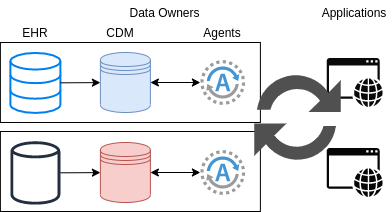
\includegraphics[width=.6\textwidth]{overall-arch-v1}
    \caption{High-level architecture of the extraction and update process.}
    \label{fig:overall-arch-v1}
\end{figure}

\section{Requirement Analysis}

When we enter the realm of accessing an institution's sensitive data, some problems start to arise.
Not all data owners are willing to, or legally can't, provide direct access to their data.
When building this part of the system, we have to consider this and have several options available that use different levels of access and according to the demands of each specific data owner, use the most appropriate one.
In one end, a single solution could have full access to the data, extracting the metadata directly from the original data.
At the other end of the scale, the burden of extracting data is removed from us and the system is dependent on the data owner providing the metadata and only then the system processes the metadata.
Having several options for different access levels is more flexible, however, it requires maintaining several tools which are not reliable.
A more appropriate alternative is to have a single option, that is designed considering the most strict access to the data, however, we still need to provide a tool to extract the metadata.
The only difference is that we are not the ones executing it.

As the extracting tool has direct access to the data, using an existing and widely known tool is a must, so data owners are inclined to use it.
Additionally, making fewer to no changes is preferable to ensure that data owners don't discard the tool because they don't trust the changes.

\begin{figure}[H]
    \center
    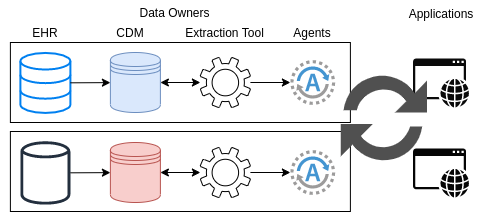
\includegraphics[width=.6\textwidth]{overall-arch-v2}
    \caption{High-level architecture of the extraction and update process}
    \label{fig:overall-arch-v2}
\end{figure}

In figure \ref{fig:overall-arch-v2} is presented the overall architecture of the system, where the agent is the tool in charge of parsing the metadata provided by the data owner, which is then sent to the applications.
Regarding this last point, there needs to be a way for the data to go from the agents to the applications.
One ambitious solution is to create a decentralized peer-to-peer network of agents, avoiding developing a central component.
In such solution, the agents are in charge of managing and sending the data to the applications.
However, data owners might not want to spend their hardware resources to maintain a network.
Since the agents are executed on the data owner's system, they should do only the required and minimal functionality, spending the few resources as possible.

A more executable solution is to have an intermediate component that receives the metadata from the agents and then distributes that data across the applications, following a centralized network architecture as it is presented in figure \ref{fig:overall-arch-v2}.

\begin{figure}[H]
    \center
    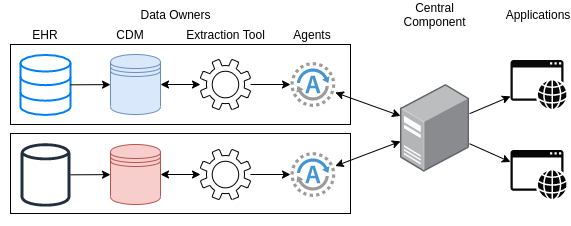
\includegraphics[width=.6\textwidth]{overall-arch-v3}
    \caption{High-level architecture of the extraction and update process, with a centralized network approach.}
    \label{fig:overall-arch-v3}
\end{figure}

This central component will be used to manage the data and the applications to where such has to be sent.
However, it is also crucial that feedback is provided on the system's state, such as how the data is flowing, which applications received which data, and which databases sent data into the system.

% aqui digo que percisamos de um componente intermedio. mais á frente vou dizer que percisamos um componente intermedio entre o kafka e as aplicações. coisas diferentes

On the applications side, there are other important factors to consider before going forward on implementing the intermediary component mentioned before.
First, then we talk of application we are considering only web application that expect to receive metadata through a \gls{rest} \gls{api}.
Second, the \gls{api}s of different applications expect the metadata in distinct arrangements.
A way out of this would be to specify a set of endpoints that each application had to implement, yet that would lead the applications to have two sets of endpoints that do the same thing.
On the other side, making a flexible option, where the requests where the data is sent are customizable, would be more appealing for the target applications, which would not have to make any changes.
Third, not all applications require all metadata data that is extracted from a database.
Some use all the data, others only need a value of such data.

\subsection{Functional Requirements}

\begin{enumerate}
    \item Databases must be registered on the central component
        \begin{list}{}{}
        \item By having a record of the databases that are attached to the network, the system can avoid accepting data from databases that were not registered in the system.
        \end{list}

    \item It must be possible to check what agents are active at a certain point
        \begin{list}{}{}
            \item This allows giving feedback on the state of the network to the admin.
        \end{list}

    \item The system should allow managing the destination applications
        \begin{list}{}{}
            \item The applications to where the data of the databases are sent, should not be hard-coded, for that, the network admin should be able to perform \gls{crud} operations on such.
                The term application should be interpreted as web applications that have \gls{rest} \gls{api} endpoints available to receive data.
        \end{list}

    \item The system should provide statistics on the data that has circulated
        \begin{list}{}{}
            \item This is yet another feature to give feedback to the network admin about, now allowing to both check the amount of data that each database sent, and the amount of data that each application received.
        \end{list}

    \item The format of the request sent with the metadata to each application must be customizable
        \begin{list}{}{}
            \item This is important since different applications expect to receive metadata in distinct formats since each application has a different \gls{api}.
        \end{list}

    % eu não falo aqui das pipelines, que permitem filtrar os dados, pk isso foi algo que adicionei como consequencia consequencia em termos usado kafka

    \item The system should allow to group Databases
        \begin{list}{}{}
            \item In a scenario where both all the destination applications and all databases belong to the same project, the metadata of the databases makes sense in all applications.
            \item Now consider a scenario where half of the databases are associated with one project and the rest with another.
          Each project has a destination application that receives the data.
          Considering that there is no concept of project or groups, both applications will receive data of both projects.
          To solve this, it required to have two installations of this system, one for each project.
          By grouping databases, data of a database can be guided to applications that are also attached to the same group.
        \end{list}

\end{enumerate}

\subsection{Non-Functional Requirements}

\begin{enumerate}
    \item The data owner can stop the agent at any time
        \begin{list}{}{}
            \item This was also applied in \cite{gaain}.
                It gives yet another layer of control to the data owners over their data.
          If at any time, they don't want to share their data, they can stop the agent.
          This also poses a constraint in the system that it should not be designed assuming that the agents, once deployed, will always stay active.
        \end{list}

    \item The extraction tool should be based as much as possible on an already existing solution
        \begin{list}{}{}
            \item Using a working solution avoids having to build a new tool from scratch.
              But apart from that, using a known solution as a base helps to gain the confidence of the data owners so that they use the resulting solution in their databases.
        \end{list}

    \item The agents must not have direct access to the data
        \begin{list}{}{}
            \item This option assumes the least amount of access to the user's data so data owners are receptive to allow agents to be run on their local deployments.
              This will require that an agent has access to at least a shared storage where agents check for new data and data owners post their extracted metadata.
        \end{list}

    \item The agent should easily deployable
        \begin{list}{}{}
            \item As the installation of the agent will be done by a person not familiar with the project, this process should be as smooth as possible and well documented.
        \end{list}

    \item Agents should spend few resources
        \begin{list}{}{}
            \item Considering agents run on data owners' deployment environment, it should have a low resource footprint so it does not impose any disruption.
              For that, they must be designed to perform only the required task.
        \end{list}

    \item The system should not require any open ports on the data owners' deployment environment
        \begin{list}{}{}
            \item As there might be communication between the central component and the agents, requesting an open port on the data owners' deployment environment might not be possible since it could require them to change firewall settings as was mentioned in \cite{popmednet}.
        \end{list}

    \item Scalable
        \begin{list}{}{}
            \item As more databases are connected to the network, the system should allow increasing resources so that it handles processes faster.
        \end{list}

    \item Microservice architecture
        \begin{list}{}{}
            \item The system should be composed of simple and replaceable components that deal with well-defined tasks.
        \end{list}
\end{enumerate}

\subsection{Use Cases}

From the previous requirements defined, there can be outlined two actors that will interact with the system:

\begin{itemize}
    \item Data owners, which maintain the agent on their local deployment;
    \item System admin, that interacts with the central component to manage the whole system.
\end{itemize}

In figure \ref{fig:use-cases} is presented the use-case diagram, which shows the actions that each actor performs on the system.
Such actions were divided into three groups: Agents, Metadata Extraction, actions on the central component related to receiving data from the agents, and Metadata Update, actions on the central component related to sending data to the applications.

\begin{figure}[H]
    \center
    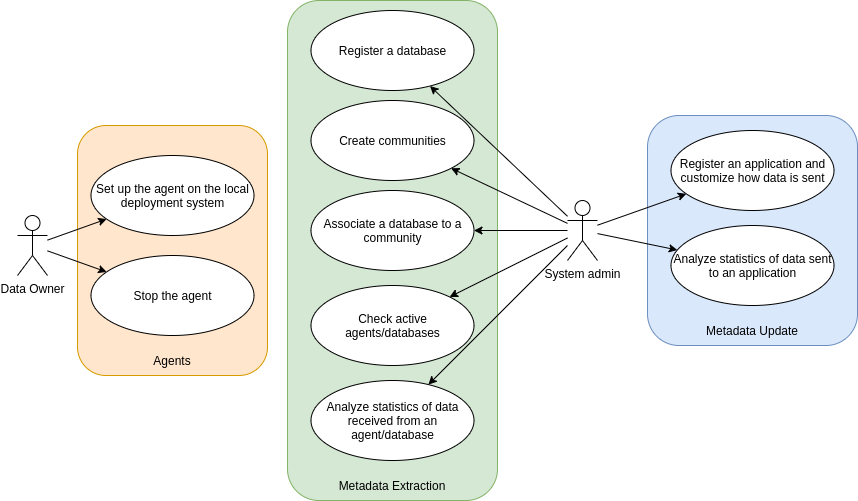
\includegraphics[width=\textwidth]{use-cases}
    \caption{Use case diagram of the metadata extraction and update system}
    \label{fig:use-cases}
\end{figure}

\begin{enumerate}
    \item Set up the agent on the local deployment system
        \begin{list}{}{}
            \item Since it's not expected that data owners provide access to their deployment environment, the responsibility to set up the agent is imposed on them.
        \end{list}

    \item Stop the agent
        \begin{list}{}{}
            \item As Data owners control their data and the access to it at all times, them stopping the agent should be an action expected by the system.
        \end{list}

    \item Register a database
        \begin{list}{}{}
            \item As new databases enter the network and agents are deployed to gather their metadata, the system admin needs to register new databases on the central unit, so the data received is accepted into the system.
        \end{list}

    \item Create communities
        \begin{list}{}{}
            \item In a scenario where there are several databases from distinct projects, there is the need to group databases to treat their data separately.
        \end{list}

    \item Associate a database to a community
        \begin{list}{}{}
            \item Once there are databases and communities registered in the system, the system admin can do many-to-many associations between them.
        \end{list}

    \item Check active agents/databases
        \begin{list}{}{}
            \item At any time, the system admin can check the state of the network and verify which databases have an agent active.
        \end{list}

    \item Analyze statistics of data received from an agent/database
        \begin{list}{}{}
            \item As agents send data to the central component of the network, statistics can allow the system admin to see what databases contribute more data to the network and its frequency.
        \end{list}

    \item Register an application and customize how data is sent
        \begin{list}{}{}
            \item The system admin will also define the destination applications for the data received from the agents, setting also the format of the request that sends the data to such applications.
        \end{list}

    \item Analyze statistics of data sent to an application
        \begin{list}{}{}
            \item As metadata enters the system, having statistics of data sent to the application helps check if the system is working properly and if the applications are receiving the expected data.
        \end{list}

\end{enumerate}

\section{Metadata Extraction}

With the requirements analysis done, let's first go over the portion of the system which executes in data owners' space.

\subsection{ACHILLES}
% percisade de um vocab files
% escolhemos principalmente por estar direcionada para bases de dados cdm
% organização interna
% implementado em R
% diferentes maneiras de exportação (json, csv ou diramente para db)
% a query for each analaysis
% Catalogue Export

Regarding the extracting tool, from the ones presented in chapter \ref{chapter:background}, the most indicated for our use case is \gls{achilles}, developed by \gls{ohdsi}, or a variation of such.
This choice was mainly because of its database, instead of the dataset, focused design, and because it was built to extract metadata from databases that follow the \gls{omop} \gls{cdm}.

The most adequate option is Catalogue Export~\cite{peters-tool} which was built using \gls{achilles} as the base, the main difference being that it only exports the required data to the \gls{ehden} project.

These tools are distributed as an R\footnote{https://www.r-project.org/} package, which uses a set of third-party packages that allow the extraction of metadata from different \gls{rdbms}s.
Metadata is separated into analyses, where each one captures a specific metadata metric of the database.
Each analysis is captured through a different \gls{sql} query, allowing to extract all analyses through a multithreading approach.
To make use of the package, the user must provide the information to connect to the database, such as user and password, an output directory to export the results, and the name of three schemas, which are, in most \gls{rdbms}s, a way to group tables within a database within the \gls{rdbms}.
The schemas to provide are:

\begin{itemize}
    \item \gls{cdm} Data: where the original \gls{cdm} data is stored;
    \item Results: that contains the tables that store the results obtained from the execution of analyses queries;
    \item Vocabularies: as each clinical database certainly will contain their distinct internal representation of clinical concepts, such as a database might encode sex with just a character (f, m, o), others might encode with the whole word (female, male, other), the \gls{omop} \gls{cdm} makes use of standardized vocabularies that allow creating a homogeneous representation for different databases.
        Such vocabularies can be acquired on the \gls{ohdsi}'s ATHENA website\footnote{\url{https://athena.ohdsi.org/}}.
\end{itemize}

As this R package should only perform reads on the original data, the package should use a custom user that only has read permission on the \gls{cdm} data schema.
This can also be applied to the vocabularies schemas, as the package will use it only to perform joins with the \gls{cdm} data.
Regarding the results schema, read and write permissions are required to insert the results data of the analyses queries.

The package also allows exporting the results data to a \gls{csv} file, which, on the \gls{ehden} project, is then uploaded into a plugin of \gls{ehden} Portal~\cite{ehden-portal}, which was built using the MONTRA framework, the main topic of the previous chapter, called Network Dashboards~\cite{dashboards}.
This plugin makes use of the metadata from the uploaded file to build several dashboards (figure \ref{fig:dashboards}), which allow researchers to better analyze and compare the data of clinical databases.

\begin{figure}
    \center
    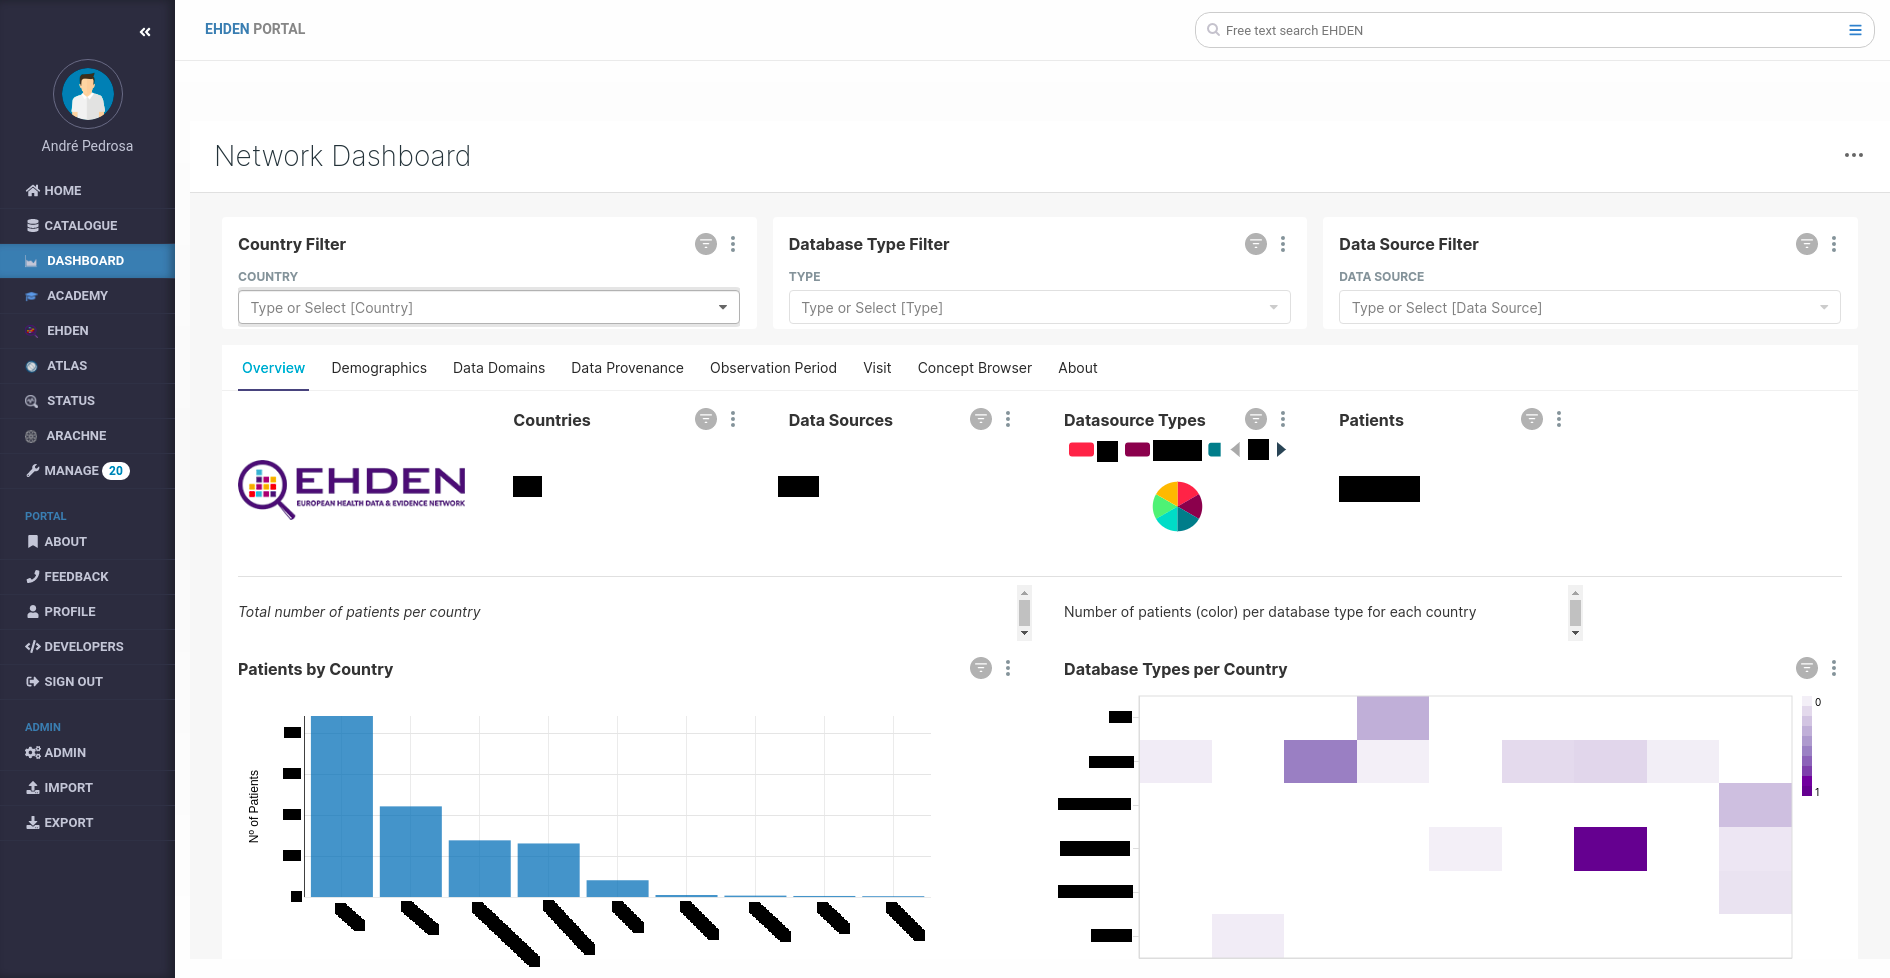
\includegraphics[width=\textwidth]{dashboards}
    \caption{Network Dashboards tool used as a plugin on the \gls{ehden} Portal}
    \label{fig:dashboards}
\end{figure}

\subsection{Publish-subscribe Systems}

During the requirement analysis, one of the non-functional requirements was that ``The system should not require any open ports on the data owners’ deployment environment''.
This implies that the request of communication must be from the agents to the central component, as the contrary can only be achieved if the agent is listening on an open port.
However, data still has to flow from the central component to the agents, such as if the central component wants to know if an agent is active.
One solution would be to have a persistent connection between both ends, however, this could overload the central component if a high number of databases enter the network and it would be continuously taking resources from the data owner's system.

An alternative is to follow a pull philosophy.
The central component can put requests on a message queue, the agent checks periodically this queue and if it finds any request, responds to it.
This can be interpreted as following the publish-subscriber pattern.
This solution also aids achieve the ``Microservice architecture'' non-function requirement as it helps decouple services since they do not require to be aware of each other.
Additionally, the publisher service will not necessarily block waiting for the subscriber service to receive the message, also known as an asynchronous message system.

There are two well know and widely used implementations of such systems: RabbitMQ and Kafka\cite{kafka-vs-rabbitmq}.

\subsubsection{RabbitMQ}

It is recognized implementation of the \gls{amqp} protocol, which this last appears appeared from the need to have interoperability between distinct asynchronous messaging systems.
Before the specification of the \gls{amqp} protocol, there were already several standards for synchronous messaging, however, the asynchronous world did not have such standards.
There was the open \gls{jms}, however, it was limited to java and was simply an interface standard, not specifying a standard protocol.
\gls{amqp} defines a binary protocol implementation, ensuring interoperability between tools implementing the protocol individually.

igure \ref{fig:rabbitmq} presents the architecture of RabbitMQ/\gls{amqp}.
The message brokering responsibility is divided into exchanges and message queues:

\begin{itemize}
    \item Exchange: Accepts messages from the publishers and, based on a set of rules routes, messages to the indicated queues;
    \item Message Queue: Holds messages and sends them to the consumers
\end{itemize}

\begin{figure}[H]
    \center
    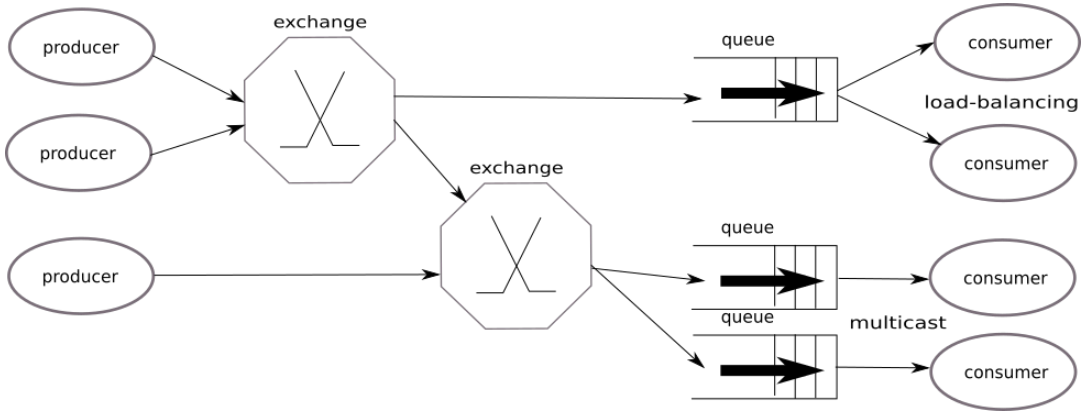
\includegraphics[width=.9\textwidth]{rabbitmq}
    \caption{RabbitMQ(AMQP) Architecture. Retrieved from \cite{kafka-vs-rabbitmq}}
    \label{fig:rabbitmq}
\end{figure}

\subsubsection{Kafka}

Kafka was built at LinkedIn, as its central event pipelining platform.
Before developing it, the team tested alternatives, such as ActiveMQ, a popular messaging system based on \gls{jms}.
However, two problems arose during production tests:
\begin{enumerate}
    \item If the queue started filling up to the point of not being able to store all the messages in memory, performance would sharply drop due to I/O;
    \item To be able to send the same data to a different consumer implies duplicating that data in another queue.
\end{enumerate}

They concluded that the explored messaging systems were designed to target low-latency use cases instead of high-volume scale-out deployment that was needed at LinkedIn.
The team decided to build their custom infrastructure that produces efficient persistence, supports several consumers with a low-performance penalty, and mainly supports distributed consumers while maintaining a real-time messaging abstraction usually obtained from messaging systems.

As a result, the produced system is a scalable publish-subscribe messaging system designed around a distributed commit log.
With this, high throughput is achieved due to data being written to log files with no immediate flush to disk, which allows to build the system with efficient I/O patterns.

The high-level architecture of Kafka is presented in figure \ref{fig:kafka}.
Producers send messages to a Kafka topic.
Each topic is distributed over a cluster of Kafka brokers, with each broker holding zero or more partitions of a topic.
A partition is an ordered append-only log of messages that are persisted in disk.
All topics are accessible for reading by any number of consumers, and new consumers have no performance penalty.
Due to its simple storage layout, every time a producer publishes a message to a topic, the broker simply appends the message to the file corresponding to the associated partition.

\begin{figure}[H]
    \center
    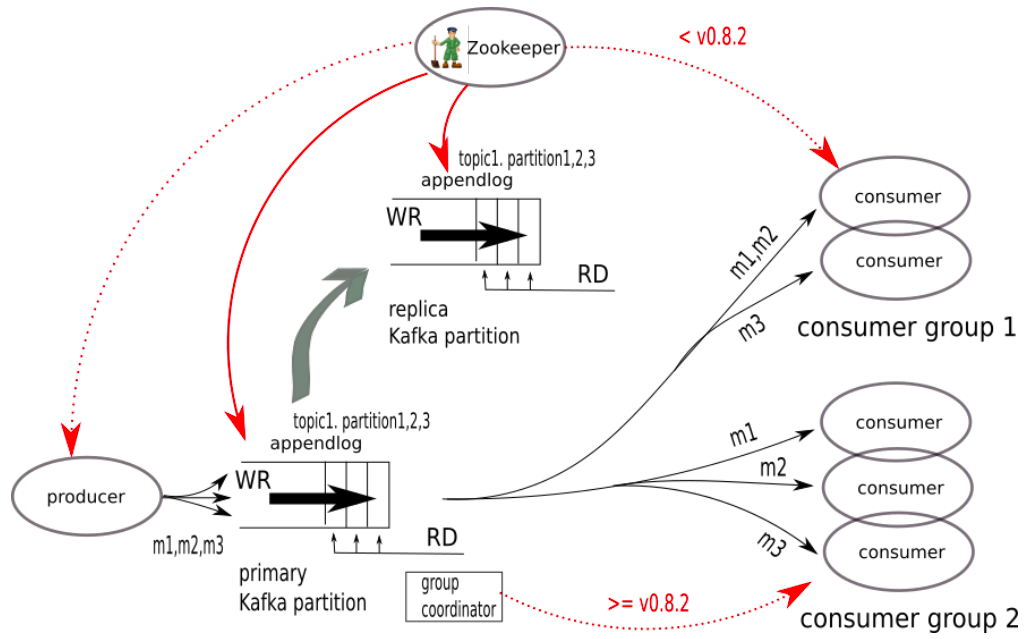
\includegraphics[width=.8\textwidth]{kafka}
    \caption{Kafka Architecture. Retrieved from \cite{kafka-vs-rabbitmq}}
    \label{fig:kafka}
\end{figure}

In contrary to the regular publish-subscriber system, the concept of a consumer in Kafka is generalized to be a group of co-operating processes running as a cluster.
Because of that, a message in a partition of a topic is delivered to only one consumer of a group.
Then, partitions allow to control the level of parallelism of consumers, as different partitions of a topic are assigned to different consumers of a consumer group.

In the end, to achieve the high-throughput requirements, Kafka went on a different road compared to the classic principles of messaging systems in several ways.

\begin{itemize}
    \item It partitions up data so that the production, brokering, and consumption of such can be handled by a cluster of entities that can be scaled as load increases;
    \item Messages are not removed from the log, instead, they can be replayed by consumers;
    \item Reader progress is maintained only by the consumers, so message deletion can only be managed based on a retention policy setting, based either on message count or age;
\end{itemize}

\par\noindent\hfil\rule{.6\textwidth}{0.4pt}\hfil

Originally, the intent was to use a publish-subscriber system just for the communication between the agents and the central component.
However, Kafka has some functionalities that appeal to use also to manage metadata, working as a central component.
Having long-term message storage allows to easily build a fault-tolerant system since consumers can easily replay the message received on a topic.
Furthermore, due to the popularity of Kafka, several libraries and frameworks were developed to extend their usage.
One of them is Kafka Connect, a framework that allows to reliably and easily stream data between Kafka and external systems.
There is also a Kafka Streams\footnote{\url{https://kafka.apache.org/documentation/streams/}} library to perform processing on streams of data on top of Kafka.
As stated before, a different application might not be expecting the entire data from the databases, for that, stream processing features could be useful to filter the data before reaching the target applications.
Finally, with its easily scalable modular architecture, Kafka is well suited to our use case.

\subsection{Kafka Source Connectors}
% kafka tem algumas appllicação ja devenvolvida que tiram dados de uma source e metem mensagem no kafka
% fetch from files or from tables
% falar nas varias opcoes consideradas. as the tables não davam tudo duma vez, e as alternativas de ficheiros não davam feedback de quando tudo ja tinah sido uploaded
% o que eu escolhi da feedback de quando todos os records estão kafka e quantos records foram escritos
% a tabela implica ter esses dados guardados sempre. em differentes runs de achilles (em que os dados têm de ser apagados) eventos falsos de deleção seriam enviados

At this point, we need to find a way to move the data extracted from the database into Kafka.
As mentioned previously, the Kafka Connect framework allows to easily import and export data between Kafka and third-party systems.
Such framework provides plugins called connectors that can be of two types: source, which brings data into Kafka, and sink, which transports data from Kafka into another system.
At this stage the source connectors are more important, however, the sink connectors will still come into use further in the system.

Since the extraction of metadata through the Catalogue Export R package is a bulk process, in other words, a set of metadata metrics are extracted from the database at once, the source connector should handle the data in the same matter.
As there is no way to know, on the central component side, when all the data is in Kafka, the connector should deal with metadata as a bounded source of data, providing some kind of feedback that all data was uploaded to Kafka.

Confluent\footnote{\url{https://www.confluent.io/}}, a streaming platform based on Kafka that aims to aid in optimizing and managing Kafka clusters, has available a search engine, Confluent Hub\footnote{\url{https://www.confluent.io/hub/}}, that allows searching for Kafka connectors and more.
The different connectors available range from known database systems (MongoDB, InfluxDB, ...) to internet protocols (\gls{http}, \gls{ftp}, ...)
In our case, considering that no other application will be running along with the agents, the only storage options available are either a single table on the data owner's relational database or a directory on the disk where metadata is placed in files.

After researching on the Confluent Hub, three connectors were found to suit the possible storage options:

\begin{itemize}
    \item \gls{jdbc} Source connector\footnote{\url{https://www.confluent.io/hub/confluentinc/kafka-connect-jdbc}}

        \begin{list}{}{}
            \item It has four different modes of capturing data from tables.
                Three of them provide incremental information, sending a message to Kafka after a row of a table or a custom query is created or updated.
                The difference between these three modes is from what columns the connector tries to infer that a row has changed.
                These are not suitable for our use case, since it treats a table as an unbounded source of data.

            \item The other mode available is bulk, which sends all the rows of a table in one go.
                However, this process isn't performed based on updates on data, instead, it is executed periodically on a configured interval.
                Furthermore, no feedback is provided after all the data is present in Kafka.
        \end{list}

    \item FileSytem Source connector\footnote{\url{https://github.com/mmolimar/kafka-connect-fs}}

        \begin{list}{}{}
            \item On the contrary to the first connector, this one uses file systems as the source to insert data into Kafka.
                Not only supports fetching files from a local file system, but also widely used cloud storage solutions such as \gls{hdfs}, Google Cloud Storage, and others.
                In our case, we would be using the local file system approach, whereby the data owner places the output files of the Catalogue Export R package on a specified directory.
                As both the extracting tool supports extracting the gathered metadata into a \gls{csv} file and the connector has a specialized reader to parse files in that format, that would be the agreed format to use.
                The connector also supports either moving or deleting files once they are entirely uploaded into Kafka.

            \item As a downside, this connector does not provide any feedback once it finishes uploading the file.
        \end{list}

    \item FilePulse Source connector\footnote{\url{https://github.com/streamthoughts/kafka-connect-file-pulse}}

        \begin{list}{}{}
            \item This connector, is similar to the previous one, as it allows to load data from files into Kafka, having the possibility to also load from other file system solutions.
                It supports reading \gls{csv} files, as it allows having a cleanup policy, which can move or delete files after they are uploaded.

            \item However, contrary to the previous connector, this one sends messages regarding the progress of the upload of the file to a separate topic.
                Not only sends when it ends but also sends the number of rows/messages that were sent into Kafka, which is ideal for our use case, as we can know when the whole file is processed if the rows go through a processing stream on Kafka.
        \end{list}

\end{itemize}

\subsection{Agent Final Architecture}
% docker to facilitae deploymente of agent (will require a little intro to docker)
% data owners should automatize (if they want) the process of achilles extracting data from their databases
% send data to kafka
% responde to health check messages
% automação da extração está nas mão do data owner mas existem ferramentas simples como o crontab que executam commandos a determinadas horas

At this point, we have all the building blocks to set up an agent and make it ready to deploy on the data owners' local system.
The agent will have two internal components:

\begin{itemize}
    \item One will be the FilePulse Source Kafka connector, which will parse the files provided by the data owners and insert their data into Kafka.
        It is important to note that both the metadata and the upload notifications use different topics for each database.
        This was decided because, otherwise, some processing would be required on gathering data of a specific upload from the main topic, that would contain messages from different uploads of different databases.
        The available \gls{csv} reader of this connector allows performing transformations on the data before sending it to Kafka.
        Such transformations include ignoring empty rows, converting values on a row, among others.
        One convenient transformation available transforms the string data of a row into a structure, so data sent in Kafka's messages values is a \gls{json} value instead of a string one.
        This avoids further on the system having to parse strings received from this connector to get a specific field from the data.

    \item The other component is the Health Check Handler.
        It is in charge of sending messages periodically, telling that the agent is active, so when the admin checks the status of the agents it gets a more updated Last Time Active metric.
        As this periodic send of ``I'm active'' messages will not be that regular, one to two times a month, the admin can request an agent to answer if it is active, and it will be this component in charge of sending a response.
        Regarding this last component, as it needs to be developed from scratch, it is a great opportunity to test new technologies that are not so commonly taught on a regular Informatics Engineering course.
        By technologies, we intend to refer to the programming languages used.
        The most popular and used ones are Python and Java, however, other programming languages appeared and are starting to gain terrain on the wap app development.
        Examples of such programming languages are Rust\footnote{\url{https://www.rust-lang.org/}} and Go\footnote{\url{https://golang.org/}}.
        According to the 2020 Stack Overflow Developer Servey~\cite{so-survey}, Rust is the most loved language among developers, and Go, in terms of most popular languages, just stands behind equivalent languages such as Python, Java and C Sharp.
        Besides behind the most loved language, Rust's ownership model, which increases memory safety with compile-time checks, is something that is not present in other languages, and newcomers will have a not-so-appealing learning curve.
        For that, the decided language to use was Go, which will also be considered for other components of the system that eventually require to be built from scratch.
        The popularity of Go mainly comes from its simplicity, as it has a C-like syntax, and for having concurrency mechanisms builtin in the language, not requiring an external library to implement such concepts.
\end{itemize}

Now the only missing part of the agent is how to deploy it.
As said in the requirement analysis, the deployment of the agent should be an easy process.
At its core, the FilePulse connector is a Java application.
With that, the agent requires that the data owner has both Go and Java runtime dependencies available so that the agent could be deployed in their local system.
This could cause problems for the data owners since he could already have these dependencies, but the wrong versions, and installing a new version could cause problems.
Also, different data owners could use a different operating system, which could change the way dependencies have to be installed, so it's hard to create install instruction that covers all the possible deployment environments.
With the emerge of cloud computing, virtualization solutions started to be used, allowing to use a single physical machine for several purposes, taking more advantage of the available hardware.
To achieve this, a software called Hypervisor sits on top of the host machine, which divides the hardware resources so that they can be used by separate virtual machines~\cite{virtualization}.
However, such virtualization technology emulates an entire operating system, on every virtual machine, which is a heavy option to deploy a simple agent.
A more convenient virtualization technology is containerization.
Such technology can be seen as a very lightweight virtual machine since a container is a package of software code with just the application to run and the necessary dependencies.
Containers are also more efficient in taking advantage of the hardware available, as portions of the hardware are not statically allocated to each container~\cite{containers}.
Containers run in an operating system as they were yet another process, but for the code running in a container, the appearance is that they are running in an isolated machine.

\begin{figure}[H]
    \center
    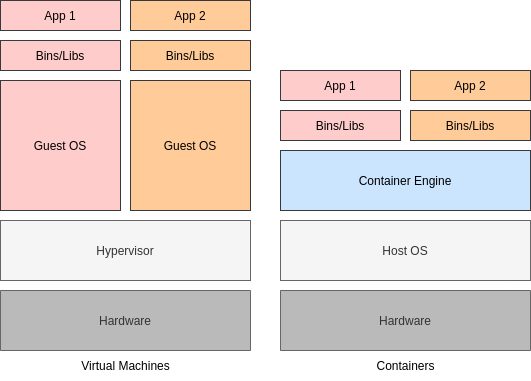
\includegraphics[width=.6\textwidth]{virtualization}
    \caption{Comparison between virtual machines and containers}
    \label{fig:virtualization}
\end{figure}

Figure \ref{fig:virtualization} presents a visual comparison between virtual machines and containers.
As can be seen, the virtual machine technology has to simulate two operating systems, in contrast to the container solution where there is only one operating system and the container engine.

With a deployment strategy in mind, figure \ref{fig:agent-architecture} shows the final architecture around the agents and pieces that connect to the data owner's system.

\begin{figure}[H]
    \center
    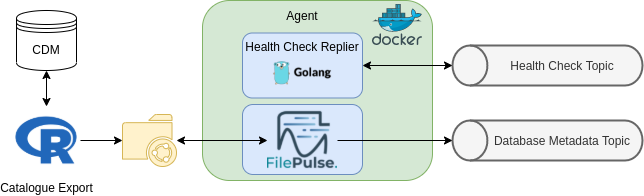
\includegraphics[width=\textwidth]{agent-architecture}
    \caption{Agent + Catalogue Extractor architecture}
    \label{fig:agent-architecture}
\end{figure}

Docker\footnote{\url{https://www.docker.com/}} is an industry standard that facilitates the process of creating, managing and sharing containers.
Developers can share their built containers, called Docker Images, in Docker Hub\footnote{\url{https://hub.docker.com/}}, which then can be used to build more specialized containers.
For example, there are official Docker images available with Python pre-installed. These images can be used by developers that want to deploy their Python apps with Docker, not having to bother installing a specific Python version.

With that, the agent will be distributed to the data owners as a Docker image.
However, data owners have to perform two tasks before starting the agent.
One is to choose which directory will be shared with the agent's container.
This can be achieved with the Docker's volume system, where a directory on the host operating system will be bound to another within the container.
The second step is to define a set of environment variables that will be unique to this agent:

\begin{itemize}
    \item AGENT\_DELETE\_CLEANUP\_POLICY: defines whether or not files must be deleted after their data is uploaded into Kafka.
        By default, the file is moved into a \textit{succed} directory, so this variable is optional.
    \item AGENT\_DATABASE\_IDENTIFIER: an identifier provided by the admin once the database is registered in the system.
\end{itemize}

After getting the Docker image of the agent, the data owners only have to execute a simple run command where defines the previous decisions:

\begin{verbatim}
docker run
  -v ./catalogue_export_files:/app/catalogue_export_files
  -e AGENT_DATABASE_IDENTIFIER=unique_db_identifier
  -d
  AGENT_IMAGE
\end{verbatim}

Next is the description of each option:
\begin{itemize}
    \item -v: binds a host directory to the one inside the container where FilePulse will read files from;
    \item -e: sets the AGENT\_DATABASE\_IDENTIFIER environment variable
    \item -d: runs the container in daemon mode
\end{itemize}

Regarding the extraction tool, we will also distribute a Docker image with the necessary dependencies preinstalled, where data owners will have to provide the necessary information for this tool to access the \gls{cdm} database and define a volume so files containing the metadata are accessible to the agent.
Concerning the automation of the extraction process, the image will contain Linux's cron command-line utility, which allows to schedule tasks.
The data owners will only have to provide the periodicity of the extraction process, using Cron's time and date syntax to define a cronjob.
\begin{verbatim}
.---------- minute
| .-------- hour
| | .------ day of month
| | | .---- month
| | | | .-- day of week
| | | | |
* * * * *
\end{verbatim}
If the extraction process were to run two times a month at three in the morning, the following configuration is used:
\begin{verbatim}
0 1 1,15 * *
\end{verbatim}
The task will execute on days 1 and 15 of every month at three in the morning.
However, if it is preferable for the data owner, he can set up his automation, or no automation, of the extraction process.

\section{Publishing}
% data is in kafka. what do we have to do to reach the applications
% idealmente usamos o kafka e afins para tudo, não tendo de desenvolver nada
% need to send custom data on a CUSTOM FORMAT to a custom REST endpoint
% Kafka Sink Connectors (The target REST API is not customizable, such as the data format ) - need for a sender application
%  https://www.confluent.io/hub/confluentinc/kafka-connect-http
%  https://docs.confluent.io/kafka-connect-http/current/overview.html
%   - envia um pedido para cada row dos dados do ficheiro
%   -  que tal dar aggregate tudo numa mensagem? resolve? não é aconselhavel ter mensagens grandes
%   - não deixa customizar body se eu quiser fazer algo {data:{patients_num:1, ...}}
% No known end on kafka topics/streams - require some management on top of kafka

At the moment, we can deploy several agents on the data owners' local systems and have a set of Kafka topics to where data is uploaded when \gls{csv} metadata files are generated.
We now need to send this data to the web application in form of \gls{http} requests.
Ideally, no other component is required, and Kafka is enough to act as a central component of our metadata publishing system.
With that, a search must be performed to find Kafka sink connectors, which should do the inverse of what the FilePulse connector does on the agent side, which is getting data from Kafka into an external system, in this case in form of \gls{http} requests.

Resorting to Confluent Hub again to search for sink connectors, only one allowed sending Kafka data in \gls{http} requests: HTTP Sink Connector\footnote{\url{https://www.confluent.io/hub/confluentinc/kafka-connect-http}}.
However, it does not meet some of the requirements.
Since different applications expect the data in distinct formats, requests need to be customizable, however, the connector does not allow to customize the request.
The data sent, will be the same as the one present on the value of the Kafka message and the connector only allows to send requests with the \gls{http}'s POST or PUT methods.

Furthermore, by default, this \gls{http} connector will send a request for each Kafka message.
The connector being used on the agent sends a message for each row of the catalogue export \gls{csv} file, which would mean that this \gls{http} connector would send several \gls{http} to an application related to the same upload.
The \gls{http} connector supports batching messages together, on the same request, however, messages are stored in memory until the batch size is not reached, which could cause memory problems if the upload contains a high number of metadata metrics and also if several databases upload at the same time.
Additionally, the number of messages sent by a database is dynamic, which the \gls{http} connector does not support, since it gathers a finite number of messages.
This problem will always exist due to the nature of Kafka, where topics can be treated as streams of data, which do not have determined start and end, and there is always data flowing.

\section{Metadata Manager}
% centralized entity working on top of kafka, dealing with the unbounded format of data in Kafka
% performs operations on top of kafka
% transforms the data to the required format
% sends to the specific application's endpoint
% 5 components

To takle the problems mentined previously, new components need to be developed.
Such group of components will be called Metadata Manager, which will perform operations on top of Kakfa.
The main issues that will be addressed are allowing to customize the requests that are sent to the applications and dealing with the unbounded factor of Kafka topics/streams.

Figure \ref{fig:metadata-manager} presents an overall architecture of how internal components of this Metadata Manager will be organized.
For the communication between components, Kafka topics are used, however their organization will be detailed when going over the several components next.

\begin{figure}[H]
    \center
    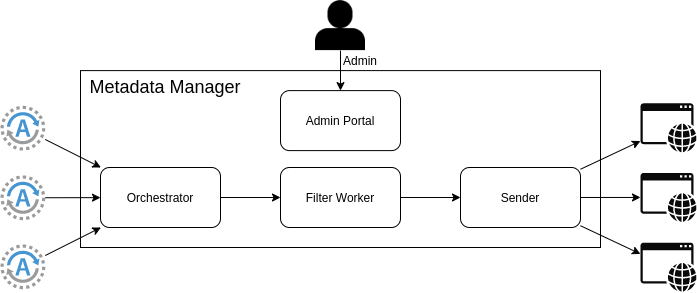
\includegraphics[width=\textwidth]{metadata-manager}
    \caption{High-level architecture of the Metadata Manager components}
    \label{fig:metadata-manager}
\end{figure}

As these components will be implemented from scratch, the programming language that will be used is Go, if applicable, for the same reason explained in the Health Check Handler component of the agent, try new emerging technologies beyond the most popular ones.

\subsection{Filter Worker}
% lets do it in go cause lets explore
% ksql introduced. easily filter data with select \_ where \_
% select and filter the data comming from the databses
% only process data of a single database at a time. handling multiple is the same is hard to handle and hard to scale
% scalable: several pipeline worker applications

Data comes from the agents in several Kafka messages, which need to be gathered together to then be used to build the custom request for each application.
As gathering all the uploaded data in memory is not a scalable option, and implementing a system with memory usage management is a complex task, the system must first filter out unnecessary data and only allow the Admin to build and send the request to the applications.
A Filter operation will remove entire rows, however, only a subset of columns might be required, for that, the system should also allow choosing which columns of the metadata are required.

That's what the Pipeline Worker component is supposed to do.
Extract only the essential data from all the data uploaded by an agent and then send it to the Sender component, who will be in charge of building and sending the request to the applications.

Since data is already in Kafka, we can take advantage of its stream processing features to filter data received from the agents.
But, once again, streams imply an unbounded size of data, so additional processing has to be built on top of such stream processing.
If a stream is created to get the data that satisfies a given condition, we need to make sure that all the uploaded data went through that given stream.
This can be achieved by creating two streams with opposite filtering conditions (figure \ref{fig:filter-workers}).
\begin{figure}[H]
    \center
    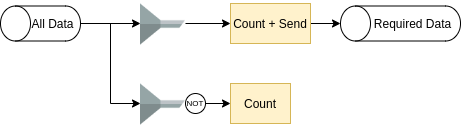
\includegraphics[width=.7\textwidth]{filter}
    \caption{How Filter Workers process unbounded data received from agents}
    \label{fig:filter}
\end{figure}
One will be used to get the actual data, the other, with the filtering condition negated, will be used just as an auxiliary.
At the end of each stream, a component will count the number of records that went through.
When both sum up to the number of messages sent by the agent, we can know for sure that all data was filtered and the Sender component can use the result data.
As the stream with the negated filtering condition will be used to just get a counter, there is no need to send the actual data on that stream, for that a single byte is sent to avoid wasting memory resources.

To develop these filtering streams, there are two options:
\begin{itemize}
    \item Kafka Streams: A Java library to process and analyze data that is already present on Kafka.
        Using it would imply implementing this Filter Worker component in Java, however, from the explanation of how a filter will be implemented, there will be several threads involved, requiring communication between them.
        Developing such an environment in Go is much easier as concurrency mechanisms are built in the language itself, and also if the number of filters gets high, threads might start to slow and use a lot of memory, as each has its own address space.
        Go, on the other hand, has goroutines, lightweight threads managed by the Go runtime, which run in the same address space.
        Using Kafka Streams would also imply that the conditions defined by the Admin, would require to be written in Java code.
    \item KsqlDB~\cite{ksql}: is a database that allows assembling stream processing applications on top of Kafka.
        It combines the power of stream processing with the known feel of a relational database through a \gls{sql}-like syntax, so stream applications can be set up with just \gls{sql} statements.
        As the data sent by the agents are messages extracted from a \gls{csv} file, the data can also be interpreted as a table, so the \gls{sql} language feats well in this case.
        It provides a \gls{rest} \gls{api} interface, so using KsqlDB does not bound the implementation to a specific language.
\end{itemize}

We opted to go with KsqlDB as it allows us to build the application in Go, taking advantage of its lightweight goroutines, allowing the system to scale better and the system to receive data from more databases.

Until now, it was assumed that each application has its filtering condition over the data.
However, two distinct applications might benefit from the same filtering condition, for that, the relationship between filters on data for an application is a one-to-many relationship, so the data resulting from one filter might be used to build and send data to several applications.

In terms of internal organization, displayed in figure \ref{fig:filter-workers}, the main goroutine is in charge of managing the several active Filters, stopping existing ones and starting new ones, according to the orders received from the Admin Portal component.
Each filter runs in a separate goroutine, which by itself launches other two goroutines.
One is in charge of counting the data that comply with the filtering condition and the other is counting the number of messages that do not fit the filter condition.
The count of messages filtered is monitored by the main goroutine of each filter.
When it reaches the number of messages that the agent sent, it tells the other child goroutines that they can stop reading from the streams, and sends a notification to the Sender component telling that data is ready to be sent.

\begin{figure}[H]
    \center
    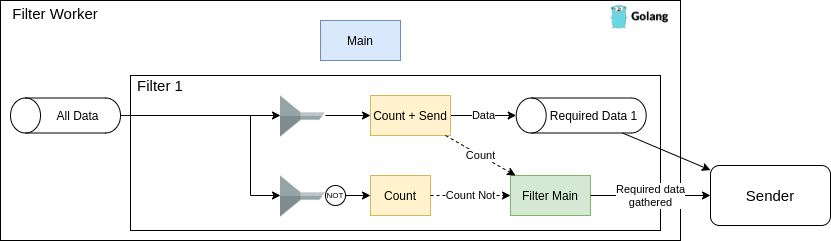
\includegraphics[width=\textwidth]{filter-workers}
    \caption{The internal organization of a Filter Worker}
    \label{fig:filter-workers}
\end{figure}

Note that the ``All Data'' topic is unique to the Filter Worker application, this means that on a Filter Worker application there can be several Filters running at the same time.
Also, this means that a Filter Worker application will obtain the data to all the filter conditions that were defined, at the same time, for one single database.
The system then allows scaling, by running several Filter Worker applications at the same time, with that, several Filters can be run for different databases at the same time.

\subsection{Orchestrator}
% why do we need this. why do not the workers read directly from the database.
%  Cause wokers use ksql, and it does not allow to create a stream and start reading at a giving time. either start or end.
% To ensure multiple records of multiple databases are not processes at the same time, this component redirects the data from databases to the pipelines workers preventing the previous problem
% why not use ksql? cant set offset to read from. either always read from start or always read from end
% why java? (only it contains a kstream api) and we use it to redirect messages from one topic to another
% 2 threads: one reads uploads and creates streams of data, another closes streams once all data was transfered

As multiple Filter Worker components might be running at the same time, there needs to be a way to redistribute the load among the running instances.
Since agents publish a topic when the upload process is done, a goroutine on each Filter Worker could dynamically create the required processing streams on the data topics of the databases that performed the upload.
However, as all data on the data topic of a database might not be related to the same upload, due to the retention policy chosen, we require to start the transmission of messages at a given offset of the data topic.
Such a thing is now achievable with KsqlDB since it only allows to read either from the latest or earliest record.
As an alternative, Kafka Streams allows achieving this.
This will require that this redistribution of work has to be written in Java, but as an advantage removes, this responsibility of reading data from databases' topics from the Filter Workers components, allowing for more concrete and small components.

Previously, it was mentioned that the concept of a consumer in Kafka is a group of co-operating processes running as a cluster, so messages of a topic are distributed in a balancing manner, sending a message to only one process of a given group.
For that, there is no need to implement a balancing algorithm to balance the data uploaded from the agents, as Kafka can achieve that already.

\begin{figure}[H]
    \center
    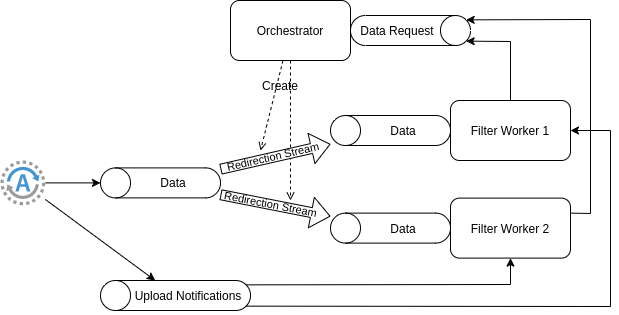
\includegraphics[width=\textwidth]{orchestrator-role}
    \caption{The workflow of how data uploaded from the agents is balanced across Filter Workers instances}
    \label{fig:orchestrator-role}
\end{figure}

As shown in figure \ref{fig:orchestrator-role}, every Filter Worker will have a consumer for the Upload Notifications topic, which all will belong to the same group.
This ensures that only one Filter Worker instance will receive a given message, thus implementing a balancing policy with Kafka.
On the Filter Worker component, another goroutine will have to be created, which will consume from the Upload Notifications topic and then broadcast this notification to the active Filters (Figure \ref{fig:filter-worker-uploads}).
\begin{figure}[H]
    \center
    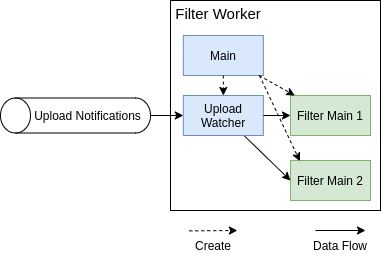
\includegraphics[width=.6\textwidth]{filter-worker-uploads}
    \caption{New ententies achitecture on a Filter Worker component}
    \label{fig:filter-worker-uploads}
\end{figure}
This new entity, Upload Watcher, will broadcast the notification using Go's channels, a built-in language feature that allows having pipes of communication between goroutines.
Additionally, this entity will also send a message to the Data Request topic, telling the Orchestrator that his Filter Worker instance is in charge of parsing the data associated with a specific upload of an agent.
The Orchestrator will then create the necessary redirection stream between the database's data topic and the specific Filter Worker instance's data topic.

Following the same balancing concept used for the Filter Workers, the same can be applied to the case of scaling the number of Orchestrators.
Different Orchestrator instances will consume from the Data Request topic belonging to the same group, balancing the work of redirecting upload data over several Orchestrator instances.

Internally, the Orchestrator is composed of two entities:
\begin{itemize}
    \item one that consumes from the Data Request topic and creates the redirection streams from databases' data topics into the Filter Workers' data topics;
    \item for each message received by the previous entity, another entity checks when all data reached the data topic of the target Filter Worker instance and closes the stream once that happens.
\end{itemize}

\subsection{Sender}
% sends/publishes the data resulting from the pipelines, to the application's endpoints
% why python? cause jinja and pandas (people know how to use)
% since data was filtered, small data is in memory now

At this point, the system contains the data required to build the requests and then send them to the applications.
It is now required to get, from the Admin, the configuration of the \gls{http} request to send the data.
An interface to build \gls{http} requests would require several components to allow customizations of the several items of an \gls{http} request: authorization, headers, method, \ldots
To allow flexibility on the configuration of the \gls{http} request, such an interface would either be too complex or some features would not be allowed to simplify the implementation of such interface.

Many programming languages have libraries that allow performing \gls{http} requests and customization is provided by passing different parameters to functions of such libraries.
Such parameters will then go over a validation process, avoiding the use of invalid values, such as sending a request with REPLACE as the \gls{http} method for example.
With that, it would be easier to make use of such libraries, and then Admins would provide the arguments for a function that performs \gls{http} requests.
The system would provide the data that resulted from a filter to the Admin, and then he would build a structure where they specify the required and additional optional parameters of an \gls{http} requests library's function.

On top of that, the request for each database within the same application might be different, one might use the URL ``http://app.com/data/db1/'' and another use ``http://app.com/data/db2/'', for that the system must provide additional data besides the data filtered, such as the database information.

Basically what the Admin needs to provide the system is a template defining the parameters to a function of an \gls{http} request library function.
On this template, the Admin can use placeholders to define where the system should insert certain data.
Django contains a template system that allows building dynamic \gls{html} pages.
The developer can write a normal \gls{html} page and then, using a special syntax, can tell where Django should insert data to fill the page.

\begin{verbatim}
<html>
  <head>
    <title>{{ app_name }}</title>
  </head>
  <body>
    <h1></h1>
  </body>
</html>
\end{verbatim}
In the example above, \{\{ \textit{app\_name} \}\} will be replaced by the value of the variable app\_name.

However, the entire Django framework is not required to build the Sender component, as the component does not require to either render pages or manage database models.
Only the templating system is required.
Fortunately, there's a Python package called Jinja\footnote{\url{https://palletsprojects.com/p/jinja/}}, which was built based on Django's template system.
It has a similar syntax to the Django Template System providing some additional features and being more pythonic.

For now, let us assume that the template will be an argument defined in each line, it would look something like this:
\begin{verbatim}
method: POST
url: http://www.app.com/data/{{ database_identifier }}/
data: {"patients_number": {{ filtered_data.get("patients_number") }}}
\end{verbatim}
On Jinja, placeholders are defined within \{\{\ldots\}\} tags, so it would look for the database\_identifier variable and execute the get method of the filtered\_data variable.

While building its template, the Admin must have access to the filtered data, which, on the example above, was exposed through a filtered\_data variable.
As data is in a Kafka topic, the system must provide an abstraction to easily access such data.
Once again, since data is extracted into a \gls{csv}, it can be interpreted as a tabular type data.
Two programming languages suited to read and manipulate data in this format are Python and R, which are widely used on data analysis applications.
R is a more specialized language than Python since is suited for statistical analysis~\cite{r-lang}, however, Python is more popular, as there are many data analysis and machine learning packages written in it.
As the Admin will mainly just want to access the data, the chosen approach was to expose the data using the Pandas Python package\footnote{\url{https://pandas.pydata.org/}}.
It contains a DataFrame data structure, which is widely used in data manipulation and analysis applications written in Python.

With Jinja and Pandas, the Admin can customize the request that sends the data to the applications, however, there is a use case that there is no possibility to achieve with this implementation.
It was mentioned previously that the \gls{ehden} project uses a separate tool as a plugin of the \gls{ehden} Portal to build visualizations allowing for better comparison between databases, which is named Network Dashboards.
Data is inserted into the tool by uploading a file into a form, which is not possible to reproduce with the current implementation.
In Python, the most popular library to perform \gls{http} requests is called requests\footnote{\url{https://docs.python-requests.org/en/latest/}}.
It contains several specific functions that allow performing any type of request.
Files can be sent with this library by passing a file pointer as one of the arguments.
In Python, a file pointer can be acquired by opening a file on disk.
With this, the system has to provide a way to allow the Admin to insert this file pointer in its template of the \gls{http} request.

To avoid having to create a parser to read a custom structure of key-value pairs where Admins define the parameters of the request, it would be ideal that the template could be generated directly into a Python data structure.
This can be achieved by running code dynamically.
When the template provided is rendered, replacing the placeholders by their values, a string value is generated.
We can then treat that string as Python code and execute it.
The system will require that this code returns Python's key-value data structure called dictionary, which can then be used to pass arguments to the requests function that performs the \gls{http} request since Python allows to provide arguments to a function with a dictionary.

Let's sum up the process of building and sending the requests to the applications (Figure \ref{fig:sender-request}):
\begin{enumerate}
    \item The Admin defines a template with placeholders;
    \item Once data is received by the Sender component, the template is rendered and a string will be generated;
    \item The generated string will be executed as a Python code returning a Python's dictionary;
    \item The dictionary is used to provide the parameters to the request function to perform the \gls{http} request.
\end{enumerate}

\begin{figure}[H]
    \center
    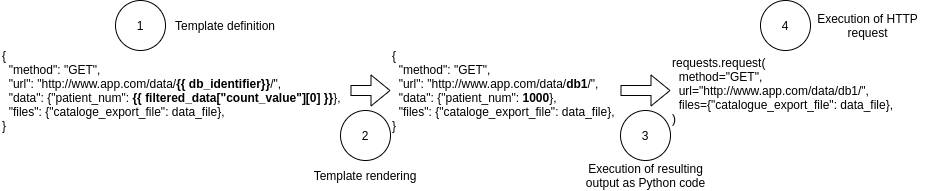
\includegraphics[width=\textwidth]{sender-request}
    \caption{Process of generating the parameters of the \gls{http} request to send to an application}
    \label{fig:sender-request}
\end{figure}

Note that, in figure \ref{fig:sender-request}, the value of the files dictionary is a variable name, which will be a local Python variable containing the file pointer to a temporary file containing the records received from the Filter Worker component.

\begin{figure}[H]
    \center
    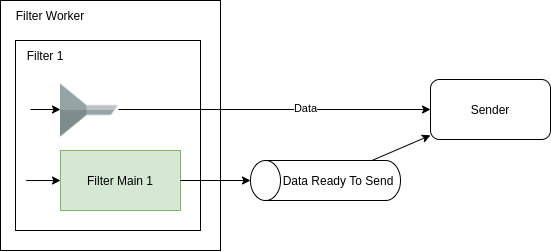
\includegraphics[width=.5\textwidth]{sender-interaction}
    \caption{Interaction between the Filter Worker and Sender components}
    \label{fig:sender-interaction}
\end{figure}

Regarding how data is transferred from the Filter Worker component to the Sender, figure \ref{fig:sender-interaction} shows a representation of the process.
Once all data was filtered, the main goroutine of each Filter will send a message to the Data Ready to Send topic with the following metadata:
\begin{itemize}
    \item Filter Worker application id: since several could be running at the same time;
    \item Filter id: through what filter did the data go;
    \item Kafka topic offset: wherein Filter's data topic does the data start.
    \item Records count: number of records that meet the filtering criteria;
    \item Database identifier: to what database does the data belong;
\end{itemize}

The internal structure of the Sender component is similar to the Orchestrator components, having the main thread consuming from the Data Ready to Send topic, and then other threads will deal with the work of building and sending the request to the applications.

Scalability is also allowed on this component as multiple Sender components can be running at the same time.
For that, consumers used by their main thread all must belong to the same group to ensure that a message is sent to only one Sender application.

\subsection{Admin Portal}
% search for tecnologies (first: golang pls . https://github.com/qor/admin)
% react or angualr allow more customizability. dont want from scratch. react-admin library
% 2 components: api backend (django) + react frontend
% manage the whole thing. talks to the other components using kafka management topics
% models and their relasionships
% Allows to perform all the use cases

Moving to the component where the Admin will use to manage the whole metadata manager.
It will allow performing the several use cases defined on the requirement analysis stage: managing communities, databases, filters and target applications, and checking statistics of the system.

As this component is mainly just a web interface, a search was performed for Go packages that allowed to create some kind of admin dashboard.
Some solutions were found such as Qor Admin\footnote{\url{https://github.com/qor/admin}} and GoAdminGroup/go-admin\footnote{\url{https://www.go-admin.com/}}.
The first solution had good documentation and features.
It creates management pages for each data model defined, allowing a user to perform the regular \gls{crud} operations on such data models.
However, there was small flexibility on what to display on a display page of a data model.
For example, if a model had an id and a name, only those fields would appear on the display page of such a model.
The second solution had better flexibility compared to the first one, however, page customization was done through a series of function calls which lead to big chunks of code to define a page, consequently, contributing to the maintainability of this component to be hard.

With this, we decided to separate this component into two parts, a web interface app and a backend app exposing an \gls{api} for the web interface app to use.
This allows using technologies that are better suited for such types of applications.
Regarding the web interface, there are several popular web frameworks/libraries such as React\footnote{\url{https://reactjs.org/}}, Angular\footnote{\url{https://angular.io/}} and Vue\footnote{\url{https://vuejs.org/}} that intend to facilitate the process of creating web applications.
However, we didn't want to build something from scratch, for that, we performed a new search for framework/libraries that used those web technologies, but were specialized to build an admin interface.
The solution found was React-Admin\footnote{\url{https://marmelab.com/react-admin/}}, a frontend framework to build data-driven applications.
React~\cite{react} is a library that allows dividing a page into components that can be reused across the web application.
Each component them as an internal state, and React will automatically update and render the associated components as the data changes.
With React-admin, customizations are easily implemented by just creating new components and then adding them to their appropriate place.
Also, such new components are implemented in a combination of \gls{html}, \gls{css} and Javascript, languages that are mainly used to build web interfaces.

Regarding the backend, the React-admin framework already takes care of the communication between the frontend app and the backend app, however, only a set of technologies are supported to use in the backend.
One of the available technologies to use is Django, which must be used alongside the framework called Django REST framework\footnote{\url{https://www.django-rest-framework.org/}}, which allows exposing Django's models through an interface.
Django was chosen over other technologies such as Springboot\footnote{\url{https://spring.io/projects/spring-boot}} or GraphQL\footnote{\url{https://graphql.org/}} due to it managing the models by itself, creating migration files every time data models definition are changed on the Django app, allowing to keep both the business logic and the stored data models in a relational database in sync automatically.
The database used here in conjuntion with Django will be PostgreSQL\footnote{\url{https://www.postgresql.org/}} since it is one of the most popular open-source and free \gls{rdbms}.

With this integration between the frontend app and the backend app set up by React-admin, when defining a page on the front end app, it is only necessary to define to which model is referred to, and then enumerate the wanted fields that must be displayed on the page.
There is no need to implement calls to the \gls{api} exposed by the backend app, as the React-admin framework will take of this automatically.
Additionally, this framework supports relationships, which allows displaying extra data associated with a model, for example, if a database belongs to a community we can also display the Community information on the database page.

\begin{figure}[H]
    \center
    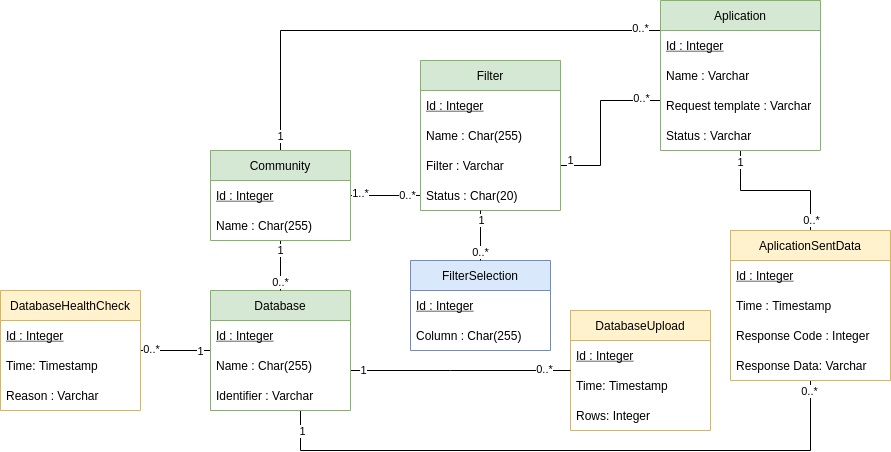
\includegraphics[width=\textwidth]{data-models}
    \caption{Data models managed on the Admin Portal component}
    \label{fig:data-models}
\end{figure}

Concerning the models' organization, figure \ref{fig:data-models} shows the relationship between models of the Metadata Manager system.
Models marks with green the admin can perform all \gls{crud} operations, models in yellow are only for reading as they are created by the Statistics Recorder component, and models in blue are dependent models, which are defined when the main model is created, in this case, FilterSelection entries are created when the Admin is creating a Filter.

\subsection{Statistics Recorder}
% kafka jdbc connector?
% Listens to the kafka topics that are used along the system and transforms into persistent statistics data (sql)
% removes this responsability from the other microservices
% belongs to a separete consumer group

Finally, this last component is in charge of reading messages that are sent between the components described before and persisting some of those messages as statistics of the system, so the admin can consult them on the Admin Portal.
This could also be done on the components that send those messages, however, this way, such components are simpler and have well-defined objectives.

To avoid interfering with the data flow of other components, this Statistics Recorder component should consume messages from the necessary topics using a different consumer group, this way Kafka will send a message of a topic to both this component and the other components.

However, there is no need to develop a component from scratch to perform this.
As we intend to move messages from Kafka into a relational database, we can make use of a Kafka Sink connector.
A connector that allows achieving this is the JDBC Sink connector\footnote{\url{https://www.confluent.io/hub/confluentinc/kafka-connect-jdbc/}}.
We are only required to set up Kafka Connect and launch a task using the JDBC Sink connector for each topic where the messages have to be persisted on the database.

\section{Summary}
% referencias para um anexo onde tem um diagrama completo do sistema
% sistema capaz de automatizar o processo de atualizar metadtados nas apps

This chapter it was explained the entire development process around a system capable of automating the procedure of updating metadata stored on web applications about clinical databases.
A solution was provided to the data owners to automatize the process of extracting metadata from their databases and then the system will make sure that that data will reach the desired web applications.
A complete diagram of the system is present in Appendix \ref{appendix:a}.

%The next chapter will present the system developed in this chapter in action, using an installation of the Montra framework improved in chapter \ref{chapter:metadata-visualization} as a target web application of the metadata.
